%7_continuous_random
%notes for the course Probability and Statistics COMS10011
%taught at the University of Bristol
%Conor Houghton conor.houghton@bristol.ac.uk
%To the extent possible under law, the author has dedicated all copyright
%and related and neighboring rights to these notes to the public domain 
%worldwide. These notes are distributed without any warranty. 

\documentclass[11pt,a4paper]{scrartcl}
\typearea{12}
\usepackage{graphicx}
%\usepackage{pstricks}
\usepackage{listings}
\usepackage{color}

\newif\ifind
\indtrue

\lstset{language=C}
\usepackage{fancyhdr}
\pagestyle{fancy}
\lfoot{\texttt{coms10011.github.com/COMS10011}}
\lhead{COMS100011 7\_continuous\_random - Conor}
\begin{document}

\section*{7 Continuous random variables}

In the case of a discrete random variables we started with outcomes
$P(e)$ which is the probability that $e$ is selected; this lead to the
probablity of events $P(E)$ and then, for random variables, to the
probability $p_X(x)$, which is the probability that the outcome
corresponds to the value $x$. In the case where the outcomes are
continuous, this story needs some adjustment because the probability
of a particular outcome is zero. That is because you can come
arbitrarily close to a continuous variable without equaling
it. Imagine your random variable is the height of a tree, the chance
of the tree being exactly six metres tall is zero, when you measure
it, it might be 6.1m or 6.01m or 5.999m or six metres and three yocto
metres, but the chance is it exactly six metres is zero. In fact, if
we were to do this experiment, measuring trees, we wouldn't mean
exactly exactly six metres, we would mean six metres within some
percision, say within a centimetre $P(H\in [5.99,6.01])$ and this is
does make sense.

There are two approaches to dealing with this; the first is to define
the \textbf{distribution function} or \textbf{cumulative}
\begin{equation}
F(x)=P(X<x)
\end{equation}
and we then define the \textbf{density function}
\begin{equation}
f(x)=\frac{dF}{dx}
\end{equation}
or we start with the density function and define the cumulative as
\begin{equation}
F(x)=\int_{-\infty}^x f(y)dy
\end{equation}
Obviously 
\begin{equation}
\lim_{x\rightarrow \infty}F(x)=1
\end{equation}
or conversely 
\begin{equation}
\int_{-\infty}^\infty f(y)dy=1
\end{equation}
Now
\begin{equation}
P(x\in [x_1,x_2])=P(x\le x_2)-P(x<x_1)
\end{equation}
For a continuous variable we don't have to be careful about the
distinction between $x<x_2$ and $x\le x_2$. Hence
\begin{equation}
P(x\in [x_1,x_2])=F(x_2)-F(x_1)
\end{equation}
or
\begin{equation}
P(x\in [x_1,x_2])=\int_{x_1}^{x_2} f(y)dy
\end{equation}

Obviously if $x>y$ then $F(x)\ge F(y)$, adding more outcomes can't reduce the probability. This means that $F(x)$ is a non-descreasing function and hence has a non-negative derivative, so
\begin{equation}
  f(x)\ge 0
\end{equation}
However, while all probabilities have to be less than one:
\begin{equation}
  P(x\in [a,b])=\int_a^bf(y)dy\le 1
\end{equation}
this doesn't mean $f(x)$ itself is bounded by one; it can exceed one
provided its integral over any limit is less than one. We will see
examples of this when we look at the Gau\ss ian distribution.

We can see when the density is called the density; it is very similar
to working out mass, say you had a rod with variable density $\rho(x)$
where $x$ is where you are along the rod. It wouldn't make sense to
ask the total mass of the rod at a point $x$, that would be zero, but
we could work out the mass of the rod between two points $x_1$ and
$x_2$; you'd calculate that by integrating the density.

The simplest example is a constant distribution where the outcome is
equally likely within some interval. This means that the probability
over a subinterval is proportional to the length of the
subinterval. Thus, say the interval is $[-1,1]$:
\begin{equation}
f(x)=\left\{\begin{array}{ll}\frac{1}{2}&x\in [-1,1]\\0&\mbox{otherwise}\end{array}\right.
\end{equation}
This function and the corresponding cumulative is shown in Fig.~\ref{fig_const}.

\begin{figure}
\textbf{A}
\begin{center}
% GNUPLOT: LaTeX picture with Postscript
\begingroup
  \makeatletter
  \providecommand\color[2][]{%
    \GenericError{(gnuplot) \space\space\space\@spaces}{%
      Package color not loaded in conjunction with
      terminal option `colourtext'%
    }{See the gnuplot documentation for explanation.%
    }{Either use 'blacktext' in gnuplot or load the package
      color.sty in LaTeX.}%
    \renewcommand\color[2][]{}%
  }%
  \providecommand\includegraphics[2][]{%
    \GenericError{(gnuplot) \space\space\space\@spaces}{%
      Package graphicx or graphics not loaded%
    }{See the gnuplot documentation for explanation.%
    }{The gnuplot epslatex terminal needs graphicx.sty or graphics.sty.}%
    \renewcommand\includegraphics[2][]{}%
  }%
  \providecommand\rotatebox[2]{#2}%
  \@ifundefined{ifGPcolor}{%
    \newif\ifGPcolor
    \GPcolorfalse
  }{}%
  \@ifundefined{ifGPblacktext}{%
    \newif\ifGPblacktext
    \GPblacktexttrue
  }{}%
  % define a \g@addto@macro without @ in the name:
  \let\gplgaddtomacro\g@addto@macro
  % define empty templates for all commands taking text:
  \gdef\gplbacktext{}%
  \gdef\gplfronttext{}%
  \makeatother
  \ifGPblacktext
    % no textcolor at all
    \def\colorrgb#1{}%
    \def\colorgray#1{}%
  \else
    % gray or color?
    \ifGPcolor
      \def\colorrgb#1{\color[rgb]{#1}}%
      \def\colorgray#1{\color[gray]{#1}}%
      \expandafter\def\csname LTw\endcsname{\color{white}}%
      \expandafter\def\csname LTb\endcsname{\color{black}}%
      \expandafter\def\csname LTa\endcsname{\color{black}}%
      \expandafter\def\csname LT0\endcsname{\color[rgb]{1,0,0}}%
      \expandafter\def\csname LT1\endcsname{\color[rgb]{0,1,0}}%
      \expandafter\def\csname LT2\endcsname{\color[rgb]{0,0,1}}%
      \expandafter\def\csname LT3\endcsname{\color[rgb]{1,0,1}}%
      \expandafter\def\csname LT4\endcsname{\color[rgb]{0,1,1}}%
      \expandafter\def\csname LT5\endcsname{\color[rgb]{1,1,0}}%
      \expandafter\def\csname LT6\endcsname{\color[rgb]{0,0,0}}%
      \expandafter\def\csname LT7\endcsname{\color[rgb]{1,0.3,0}}%
      \expandafter\def\csname LT8\endcsname{\color[rgb]{0.5,0.5,0.5}}%
    \else
      % gray
      \def\colorrgb#1{\color{black}}%
      \def\colorgray#1{\color[gray]{#1}}%
      \expandafter\def\csname LTw\endcsname{\color{white}}%
      \expandafter\def\csname LTb\endcsname{\color{black}}%
      \expandafter\def\csname LTa\endcsname{\color{black}}%
      \expandafter\def\csname LT0\endcsname{\color{black}}%
      \expandafter\def\csname LT1\endcsname{\color{black}}%
      \expandafter\def\csname LT2\endcsname{\color{black}}%
      \expandafter\def\csname LT3\endcsname{\color{black}}%
      \expandafter\def\csname LT4\endcsname{\color{black}}%
      \expandafter\def\csname LT5\endcsname{\color{black}}%
      \expandafter\def\csname LT6\endcsname{\color{black}}%
      \expandafter\def\csname LT7\endcsname{\color{black}}%
      \expandafter\def\csname LT8\endcsname{\color{black}}%
    \fi
  \fi
  \setlength{\unitlength}{0.0500bp}%
  \begin{picture}(3600.00,2520.00)%
    \gplgaddtomacro\gplbacktext{%
      \csname LTb\endcsname%
      \put(726,743){\makebox(0,0)[r]{\strut{} 0}}%
      \put(726,1348){\makebox(0,0)[r]{\strut{} 0.5}}%
      \put(726,1953){\makebox(0,0)[r]{\strut{} 1}}%
      \put(858,220){\makebox(0,0){\strut{}-2}}%
      \put(1444,220){\makebox(0,0){\strut{}-1}}%
      \put(2031,220){\makebox(0,0){\strut{} 0}}%
      \put(2617,220){\makebox(0,0){\strut{} 1}}%
      \put(3203,220){\makebox(0,0){\strut{} 2}}%
    }%
    \gplgaddtomacro\gplfronttext{%
    }%
    \gplbacktext
    \put(0,0){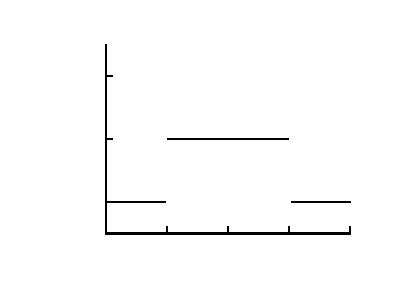
\includegraphics{fig_p_const}}%
    \gplfronttext
  \end{picture}%
\endgroup

\end{center}
\textbf{B}
\begin{center}
% GNUPLOT: LaTeX picture with Postscript
\begingroup
  \makeatletter
  \providecommand\color[2][]{%
    \GenericError{(gnuplot) \space\space\space\@spaces}{%
      Package color not loaded in conjunction with
      terminal option `colourtext'%
    }{See the gnuplot documentation for explanation.%
    }{Either use 'blacktext' in gnuplot or load the package
      color.sty in LaTeX.}%
    \renewcommand\color[2][]{}%
  }%
  \providecommand\includegraphics[2][]{%
    \GenericError{(gnuplot) \space\space\space\@spaces}{%
      Package graphicx or graphics not loaded%
    }{See the gnuplot documentation for explanation.%
    }{The gnuplot epslatex terminal needs graphicx.sty or graphics.sty.}%
    \renewcommand\includegraphics[2][]{}%
  }%
  \providecommand\rotatebox[2]{#2}%
  \@ifundefined{ifGPcolor}{%
    \newif\ifGPcolor
    \GPcolorfalse
  }{}%
  \@ifundefined{ifGPblacktext}{%
    \newif\ifGPblacktext
    \GPblacktexttrue
  }{}%
  % define a \g@addto@macro without @ in the name:
  \let\gplgaddtomacro\g@addto@macro
  % define empty templates for all commands taking text:
  \gdef\gplbacktext{}%
  \gdef\gplfronttext{}%
  \makeatother
  \ifGPblacktext
    % no textcolor at all
    \def\colorrgb#1{}%
    \def\colorgray#1{}%
  \else
    % gray or color?
    \ifGPcolor
      \def\colorrgb#1{\color[rgb]{#1}}%
      \def\colorgray#1{\color[gray]{#1}}%
      \expandafter\def\csname LTw\endcsname{\color{white}}%
      \expandafter\def\csname LTb\endcsname{\color{black}}%
      \expandafter\def\csname LTa\endcsname{\color{black}}%
      \expandafter\def\csname LT0\endcsname{\color[rgb]{1,0,0}}%
      \expandafter\def\csname LT1\endcsname{\color[rgb]{0,1,0}}%
      \expandafter\def\csname LT2\endcsname{\color[rgb]{0,0,1}}%
      \expandafter\def\csname LT3\endcsname{\color[rgb]{1,0,1}}%
      \expandafter\def\csname LT4\endcsname{\color[rgb]{0,1,1}}%
      \expandafter\def\csname LT5\endcsname{\color[rgb]{1,1,0}}%
      \expandafter\def\csname LT6\endcsname{\color[rgb]{0,0,0}}%
      \expandafter\def\csname LT7\endcsname{\color[rgb]{1,0.3,0}}%
      \expandafter\def\csname LT8\endcsname{\color[rgb]{0.5,0.5,0.5}}%
    \else
      % gray
      \def\colorrgb#1{\color{black}}%
      \def\colorgray#1{\color[gray]{#1}}%
      \expandafter\def\csname LTw\endcsname{\color{white}}%
      \expandafter\def\csname LTb\endcsname{\color{black}}%
      \expandafter\def\csname LTa\endcsname{\color{black}}%
      \expandafter\def\csname LT0\endcsname{\color{black}}%
      \expandafter\def\csname LT1\endcsname{\color{black}}%
      \expandafter\def\csname LT2\endcsname{\color{black}}%
      \expandafter\def\csname LT3\endcsname{\color{black}}%
      \expandafter\def\csname LT4\endcsname{\color{black}}%
      \expandafter\def\csname LT5\endcsname{\color{black}}%
      \expandafter\def\csname LT6\endcsname{\color{black}}%
      \expandafter\def\csname LT7\endcsname{\color{black}}%
      \expandafter\def\csname LT8\endcsname{\color{black}}%
    \fi
  \fi
  \setlength{\unitlength}{0.0500bp}%
  \begin{picture}(3600.00,2520.00)%
    \gplgaddtomacro\gplbacktext{%
      \csname LTb\endcsname%
      \put(726,743){\makebox(0,0)[r]{\strut{} 0}}%
      \put(726,1348){\makebox(0,0)[r]{\strut{} 0.5}}%
      \put(726,1953){\makebox(0,0)[r]{\strut{} 1}}%
      \put(858,220){\makebox(0,0){\strut{}-2}}%
      \put(1444,220){\makebox(0,0){\strut{}-1}}%
      \put(2031,220){\makebox(0,0){\strut{} 0}}%
      \put(2617,220){\makebox(0,0){\strut{} 1}}%
      \put(3203,220){\makebox(0,0){\strut{} 2}}%
    }%
    \gplgaddtomacro\gplfronttext{%
    }%
    \gplbacktext
    \put(0,0){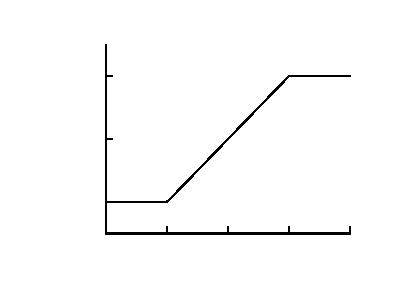
\includegraphics{fig_c_const}}%
    \gplfronttext
  \end{picture}%
\endgroup

\end{center}
\caption{The density \textbf{A} and the cumulative \textbf{B} for the distribution constant over $[-1,1]$.\label{fig_const}}
\end{figure}

The expected value is defined using the density:
\begin{equation}
\langle g(X)\rangle =\int_{-\infty}^\infty g(x)f(x)dx
\end{equation}
Hence, for the constant example:
\begin{equation}
\mu=\langle X\rangle=\int_{-\infty}^\infty xf(x)dx=\frac{1}{2}\int_{-1}^1xdx=0
\end{equation}
and
\begin{equation}
\langle X^2\rangle=\int_{-\infty}^\infty x^2f(x)dx=\frac{1}{2}\int_{-1}^1x^2dx=\frac{1}{3}
\end{equation}

This continuous version of the expected value has the same nice
properties that the discrete version did: with the obvious notation
\begin{equation}
\langle c\rangle=c
\end{equation}
and
\begin{equation}
\langle cg(X)\rangle =c\langle g(X)\rangle
\end{equation}
and 
\begin{equation}
\langle g_1(X)+g_2(X)\rangle =\langle g_1(X)\rangle +\langle g_2(X)\rangle
\end{equation}

It is useful to note that these properties can be used to see how the
mean and variance change under simple linear transformations. With the
obvious notation let $Y=X+c$, then
\begin{equation}
\mu_Y=\langle Y\rangle =\langle X+c\rangle=\langle X \rangle +c=\mu_X+c
\end{equation}
whereas
\begin{equation}
\sigma^2_Y=\langle Y^2\rangle-\mu_Y^2=\langle(X^2+2cX+c^2)\rangle-\mu_X^2-2c\mu_X-c^2=\langle X^2\rangle -\mu_X^2=\sigma_X^2
\end{equation}
Similarly, if $Y=cX$ then
\begin{equation}
\mu_Y=\langle Y\rangle=\langle cX\rangle=c\mu_X
\end{equation}
and
\begin{equation}
\sigma_Y^2=\langle Y^2\rangle -\mu_Y^2=c^2(\langle X^2\rangle-\mu_X^2)=c^2\sigma_Y^2\end{equation}

\newpage


\ifind
\section*{Summary}
\else
\subsection*{1 Probability theory}
\fi

\begin{itemize}
\item A \textbf{sample space} is a set of point, they are the possible \textbf{outcomes} of a \textbf{trial}.
\item An \textbf{event} is a subset of a sample space.
\item A \textbf{probability} is a map from events to real numbers such that
  \begin{enumerate}
    \item $P(A)\ge 0$ for all events.
    \item $P(X)=1$
    \item If $A\cap B=\emptyset$ for two events $A$ and $B$ then 
      \begin{equation}
        P(A\cup B)=P(A)+P(B)
      \end{equation}
\end{enumerate}
\item A \textbf{probability mass function} is a map from points in the sample space to real numbers such that
  \begin{enumerate}
\item $p(x)\ge 0$ for all $x\in X$
\item $\sum_{x\in X} p(x)=1$
  \end{enumerate}
\item $P(A)=\sum_{x\in A}p(x)$
\item If all the points in a sample space have the same probability then
  \begin{equation}
P(A)=\frac{\mbox{number of points in }A}{\mbox{number of points in }X}=\frac{\#A}{\#{X}}
  \end{equation}
  where $\#(A)$ means the number of points in $A$.
  \item The \textbf{binomial coefficient}
\begin{equation}
\left(\begin{array}{c}n\\r\end{array}\right)=\frac{n!}{r!(n-r)!}
\end{equation}
counts the number of subsets of size $r$ in a set of $n$ objects and 
\begin{equation}
n!=n\times (n-1)\times (n-2)\times \ldots \times 2 \times 1
\end{equation}
\end{itemize}



\end{document}




